\chapter{Problem analysis} % TODO: The title of this chapter should be similar to the title of the thesis.!

\section{The task of rendering}

In this thesis, rendering is understood as the process of obtaining an image from a description of a three-dimensional scene. A scene can be rendered in a multitude of ways, with differences both in the specifics of the initial scene description and the rendered result. The rendered visuals can range from stylized to photorealistic. Rendering happens everywhere where a computer-generated imagery (CGI) is created for a viewer to see.

The wide spectrum of possible rendering results hints at the multitude of ways in which rendering itself is performed. There are various techniques employed during the rendering process, which can be utilized together to create a desired look and fit within performance constraints. In more complex processes, there are many techniques used to render a scene, each responsible for modeling the visual aspects of different real-life phenomena or artificial effects. A renderer could be capable of adding stylized edge detection and cell-shading to an image, rendering glossy and rough surfaces, simulating shadows, reflections, caustics and refraction, dealing with hair and fur or volumetric participating media such as fog, smoke and clouds. Each of the mentioned effects can be rendered using one of many techniques, and many of them are being actively improved upon and researched.

The fact that there are many techniques currently in use to render a single type of effect creates and advantageous situation, where the techniques used can be chosen for each application depending on its characteristic. Two main factors can be discerned as defining the needs of an application: the performance requirements and the desired visual style.

The desired visual style is partially just a matter of preference defined by the style of the project. More importantly however it is a matter of clearly and efficiently conveying visual information, in a way that is consistent with the rest of the application and with what the end user expects. This means that realism, often touted the pinnacle and goal of computer graphics, is not necessarily always the best approach. A CAD (computer-aided design) application or a 3D modelling tool would be made less useful by including realistic reflections, highly contrasting full shadows and motion blur in the rendered viewport. These programs need to clearly convey information about the shape and design of 3D objects, without distractions and obstructions. On the other hand, when a player starts a modern action-adventure game, they expect a level of realism in the game's graphics that allows for immersion in the presented world. The intricate visuals also make for a more engaging experience and can mean a better reception of a game. At the same time, design choices should be made to ensure that the realism or intricacy of the presented graphics does not get in the way of enjoying the gameplay, which in the end should be the main attribute of a video game.

The performance requirements, or performance constraints, are usually better defined and divide rendering into two general categories: real-time rendering and offline rendering. When designing an offline renderer the performance constraints would most likely concern memory usage and possibly general time, or energy, efficiency, as with offline rendering the time it takes to render an image is of small importance. Most important are image quality and fidelity, often also realism. Techniques used in this context can spend as much time performing calculations as is necessary for the desired output. Offline rendering work can also easily be distributed between many machines, so-called render farms. Real-time rendering on the other hand works with very strict and small time budgets. Because a real-time application needs to be responsive to user inputs and give the illusion of continuous motion it is expected to render at least 30 frames per second (FPS), giving the time budget for a single frame of at most 0.03 seconds. This time cannot all be spent on rendering, as user inputs need to be handled and application logic performed in the same time frame. Because of that, real-time applications need to balance visual complexity and performance. They are also often created for more casual consumers than offline rendering programs, so the hardware on which the application will run is expected to be moderately powerful.

It is apparent that the choice of rendering techniques is complex and requires in-depth knowledge about each of them as early as the design stages of an application. This thesis aims to provide a guide through the rendering techniques used to render cast shadows in scenes, focusing on those applicable in real-time contexts. Some of the chosen techniques are the most widely adopted techniques, but some, while possibly less popular, are  still noteworthy due to their promised outstanding performance or visual quality. This thesis introduces the techniques, gives detailed explanations of their algorithms, shows exemplary implementations and compares them in a series of tests. The comparison is made based on measures of performance (execution time), memory consumption, visual fidelity, realism and the amount of aliasing. % TODO: what exactly will I compare?

% TODO: mention more issues more specific to shadows, that different techniques handle in different ways, such as aliasing?

\section{The role of shadows in computer generated images}

Computer graphics usually aim to reflect our surrounding reality, with techniques for rendering phenomena modeled from physical laws and after observations made in the real world. When not aiming for realism, the displayed graphics need to be at least rooted in the common human observation experience for the information to be understandable and interpretable. Shadows are a phenomenon that is very commonly present in our daily lives, deeply rooted in the common experience. An 1997 article \cite{bib:article:depth_shadows} shows that even simple shadows provide the viewer essential information on the position and movement of objects, especially movement in depth. In some cases this information even overrides other cues such as change of size due to perspective. This effect is illustrated by Fig. \ref{fig:shadow_balls_example}.

\begin{figure}[!b]
    \centering
    \begin{subfigure}{0.4\textwidth}
        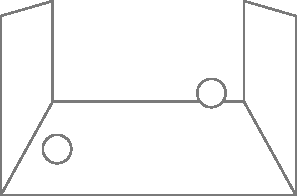
\includegraphics[width=\textwidth]{./graf/shadow_example_no_shadow.pdf}
        \caption{Shadowless scene, the positions of the spheres are ambiguous.}
        \label{fig:shadow_balls_no_shadow}
    \end{subfigure}
    \hfill
    \begin{subfigure}{0.4\textwidth}
        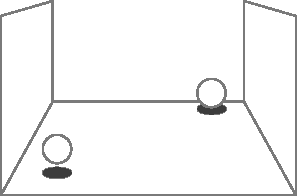
\includegraphics[width=\textwidth]{./graf/shadow_example_shadow_1.pdf}
        \caption{The upper ball seems placed on the surface.}
        \label{fig:shadow_balls_shadow_1}
    \end{subfigure}

    \begin{subfigure}{0.4\textwidth}
        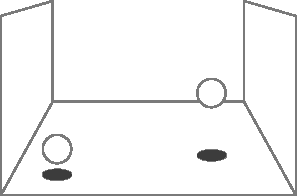
\includegraphics[width=\textwidth]{./graf/shadow_example_shadow_2.pdf}
        \caption{The upper ball seems to hover halfway.}
        \label{fig:shadow_balls_shadow_2}
    \end{subfigure}
    \hfill
    \begin{subfigure}{0.4\textwidth}
        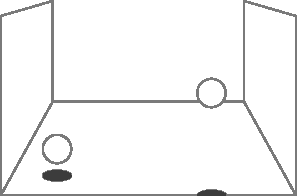
\includegraphics[width=\textwidth]{./graf/shadow_example_shadow_3.pdf}
        \caption{The upper ball seems high in the air and closer to the observer.}
        \label{fig:shadow_balls_shadow_3}
    \end{subfigure}
        
    \caption{The position and scale of the spheres do not change, yet the perceived locations in 3D space are dictated by the shadow.}
    \label{fig:shadow_balls_example}
\end{figure}
The importance of shadows for understanding the 3D composition of a scene is especially great when an observer is devoid of stereo visual information, such as in the case of observing an image displayed on a regular monitor. Shadows, lighting and perspective then become the sole sources of information about depth and the relative positions of objects in the scene.

These observations are also supported by a more recent 2018 review on the perception of shadows \cite{bib:article:shadow_perception}. It suggests more possible roles that shadows play in human perception of the world. Shadows help observers position objects in 3D space. Sometimes shadows are perceived as being a part of the object, so the lack of a shadow would make the object incomplete. Information about the shape of an object can also be derived from the shadow that it casts, as presented in Fig. \ref{fig:shadow_shape_example}.

\begin{figure}[h]
    \centering
    \begin{subfigure}{0.4\textwidth}
        
\includegraphics[width=\textwidth]{./graf/shadow_example_shadow_shape_1.pdf}
        \caption{The left shape could be a sphere, the right shape could be flat, like a coin.}
        \label{fig:shadow_shape_1}
    \end{subfigure}
    \hfill
    \begin{subfigure}{0.4\textwidth}
        
\includegraphics[width=\textwidth]{./graf/shadow_example_shadow_shape_2.pdf}
        \caption{The left shape could be a cube, and the right a shape with top and bottom faces not being parallel.}
        \label{fig:shadow_shape_2}
    \end{subfigure}

    \caption{The shadow can convey information on the shape of the object. It additionally describes whether an object is placed on a surface or above it.}
    \label{fig:shadow_shape_example}
\end{figure}

The review also mentions that shadows in art, even if depicted in a way that is impossible in the real world, are an important element for an image to be perceived as realistic and of high quality. This also applies to computer graphics, making rendering shadows a necessary element for any application that requires elevated realism or sophistication of the visual presentation. The difference between a scene with and without cast shadows is presented in Fig. \ref{fig:classroom_example} It is worth noting that since observers are not great at spotting physically incorrect shadows, as is stated in the studies, so graphics programmers can utilize this fact and take liberties with the realism of their shadows. This can lead to simplifying the algorithms producing them and improving their performance, with negligible impact on the apparent visual quality.

\begin{figure}
    \centering
    \begin{subfigure}{\textwidth}
        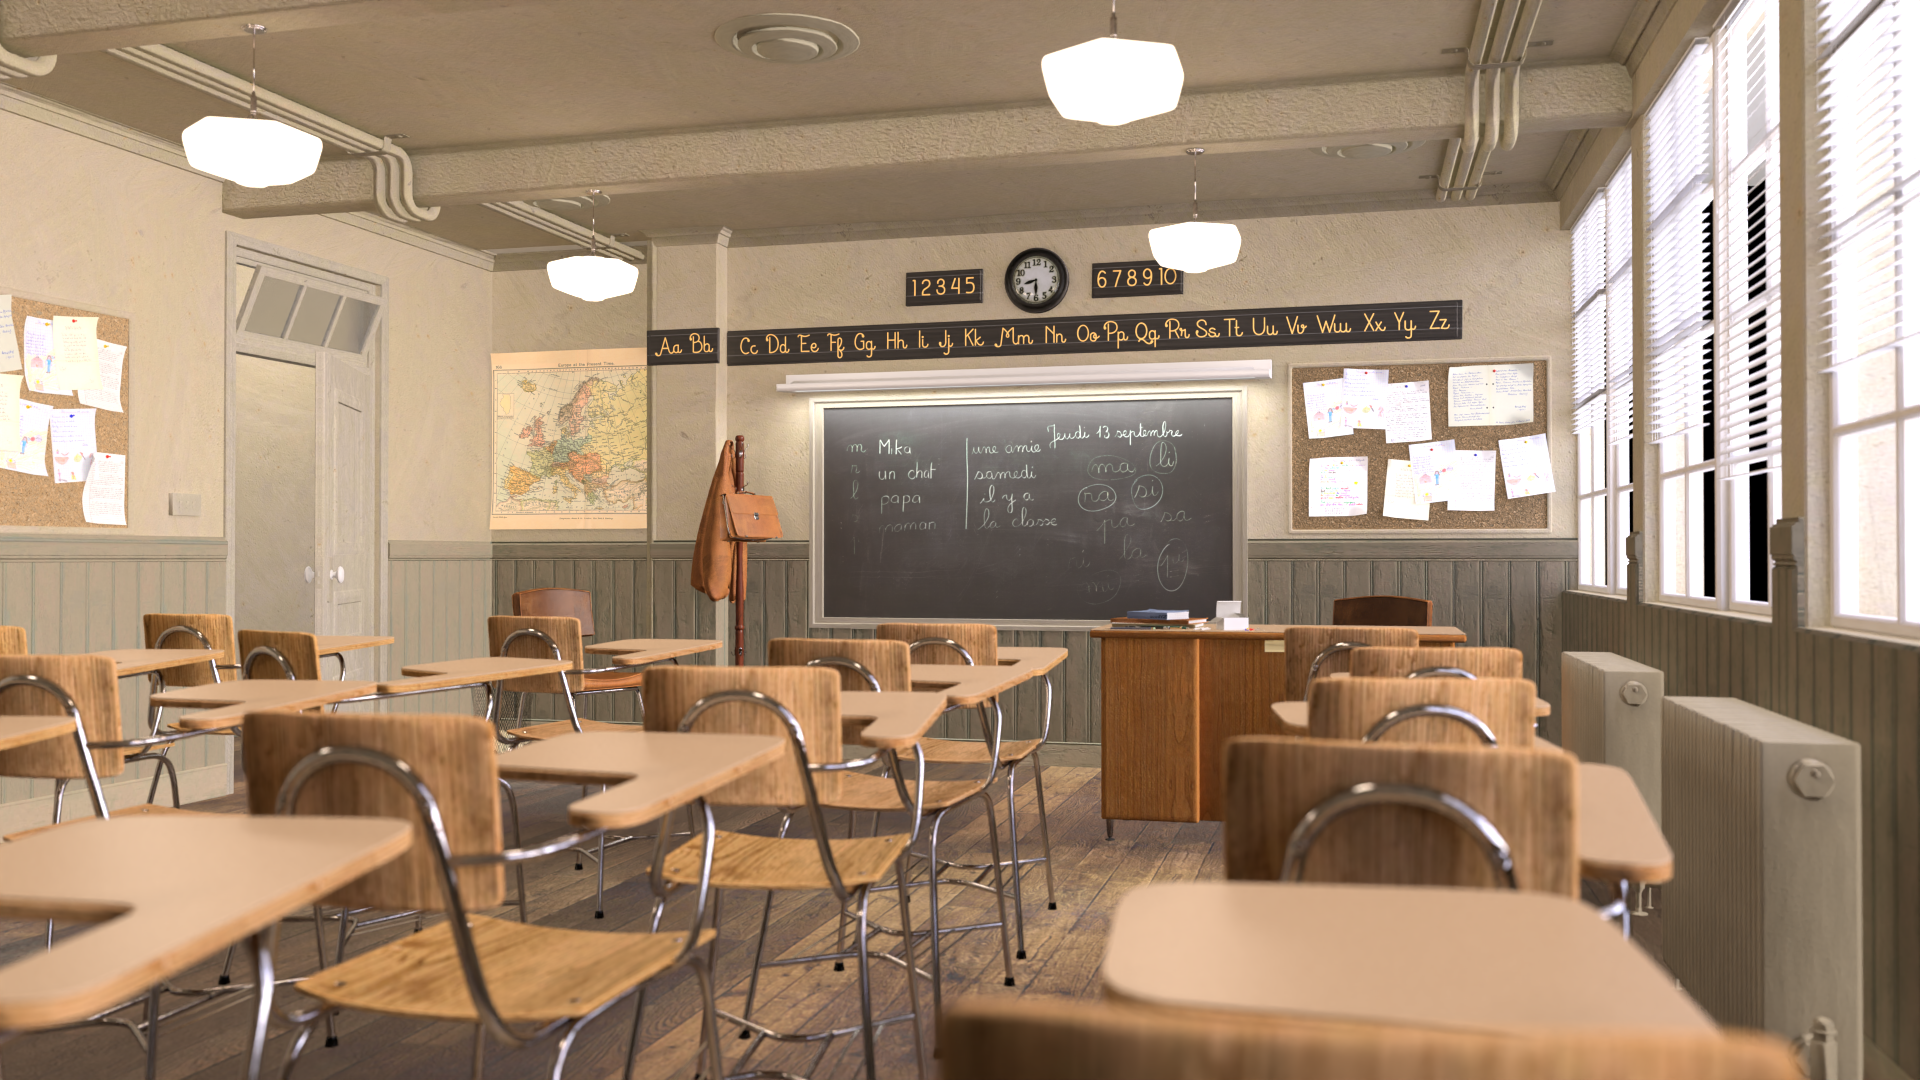
\includegraphics[width=\textwidth]{./graf/classroom_no_shadow.png}
        \caption{The scene rendered with no cast shadows, despite the high quality of models and materials, looks unrealistic and flat.}
        \label{fig:classroom_no_shad}
    \end{subfigure}

    \begin{subfigure}{\textwidth}
        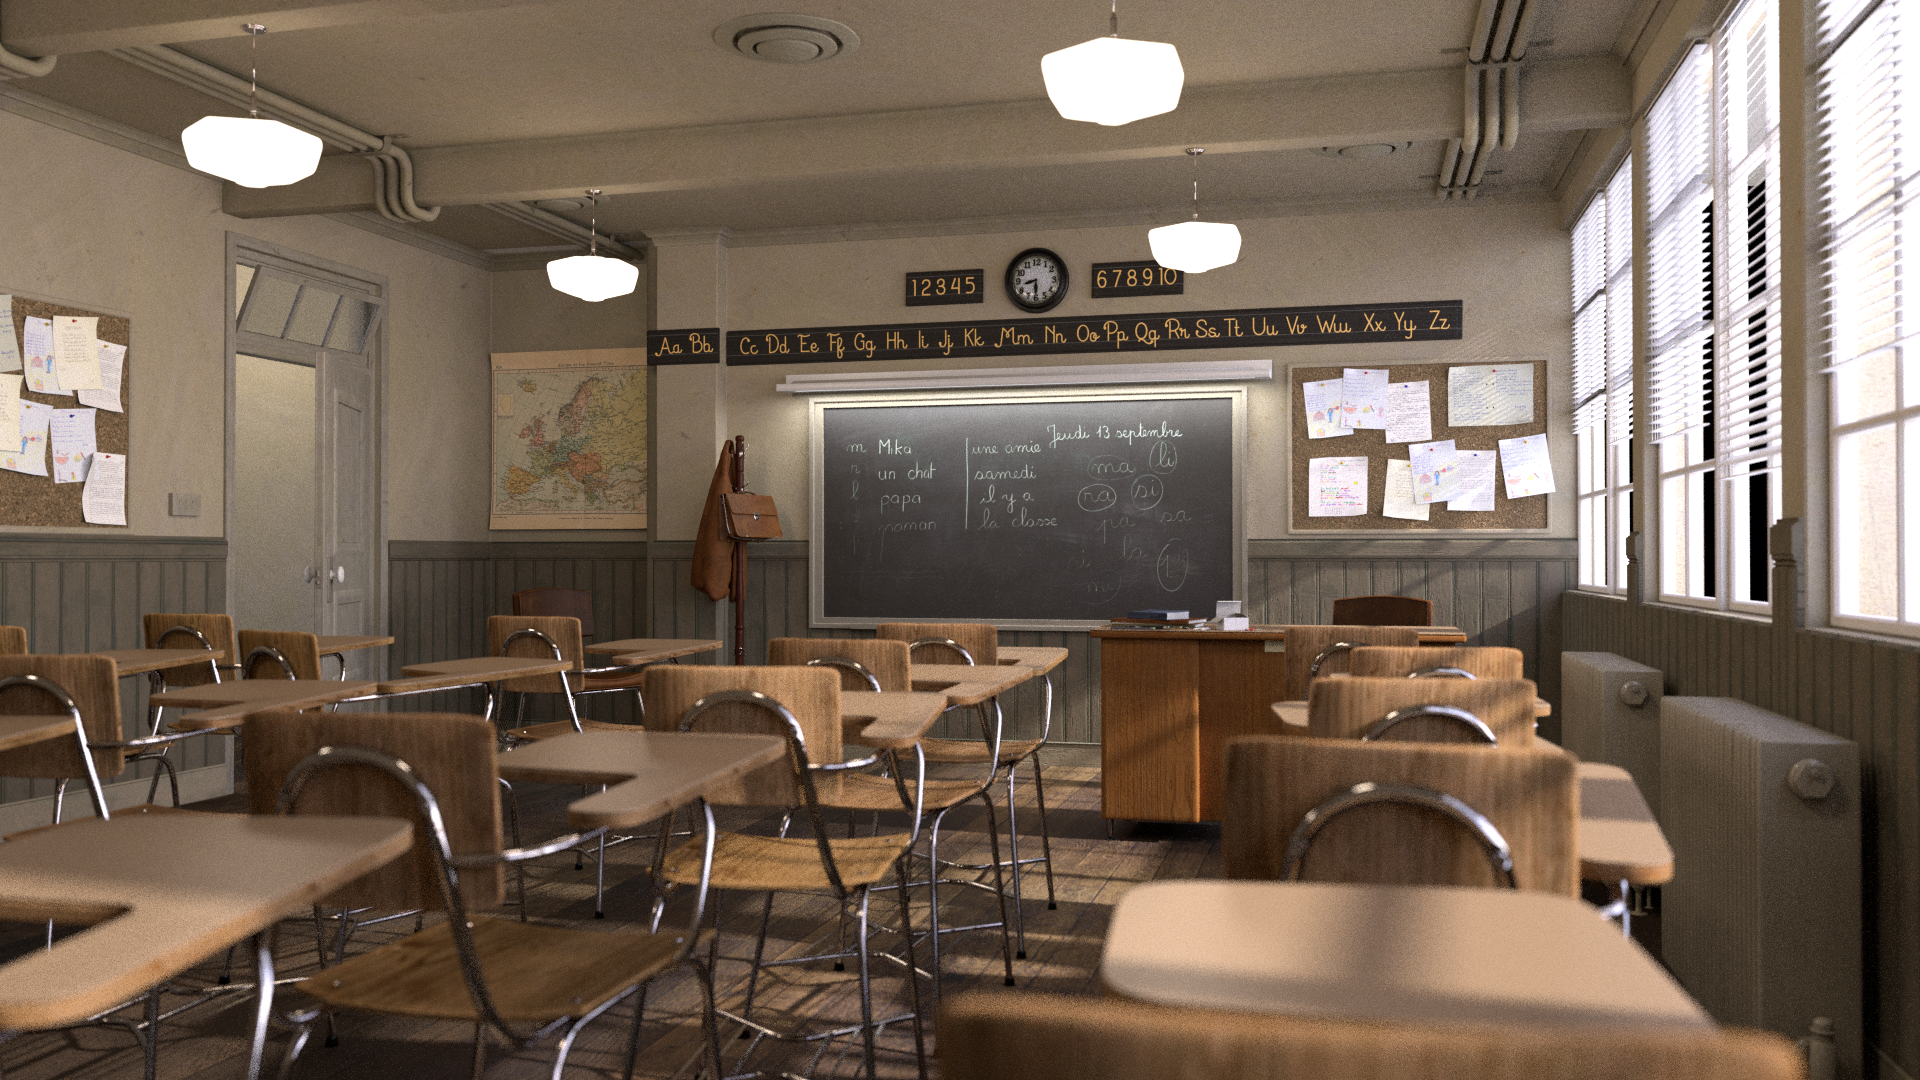
\includegraphics[width=\textwidth]{./graf/classroom_shadow.png}
        \caption{The scene rendered with cast shadows is realistic and reads well.}
        \label{fig:classroom_shad}
    \end{subfigure}

    \caption{The same scene rendered twice using Blender's Cycles renderer, with and without cast shadows. \textit{Scene source: ``Classroom'' by Christophe Seux, Blender demo files.}}
    % TODO: is this good enough for the source?
    \label{fig:classroom_example}
\end{figure}

\section{Shadow rendering techniques}

\subsection{Naming conventions}

In this thesis the term `shadows' is used interchangeably with term `cast shadows', not to be confused with shading on the surface of objects, which stems from the orientation of the surface with regard to the light source.

As presented in the ``Real-Time Rendering'' book \cite{bib:book:real_time_rendering}, a shadow is cast by a shadow caster, also called an occluder, onto a shadow receiver, when the caster occludes a line of sight from a point on the surface of the receiver to a light source.

Shadows can be differentiated into hard and soft shadows. Perfectly hard shadows are not observed in reality, as such a shadow would require an infinitely small light source. Hard shadows however are often found in computer-generated images, as they are relatively simple and cost-effective to render. Soft shadows require more complex solutions, but enhance the realism of the rendered scene. A soft shadow, as shown in Fig. \ref{fig:shadow_soft} consists of an \textit{umbra}, being the fully shadowed region, and \textit{penumbra}, meaning the region that is partially in shadow. The appearance of a soft shadow, the sizes of the umbra and penumbra defining its softness, depend on the relative distances between the shadow caster, the shadow receiver, the light source and also the size of the light source.

\begin{figure}
    \centering
    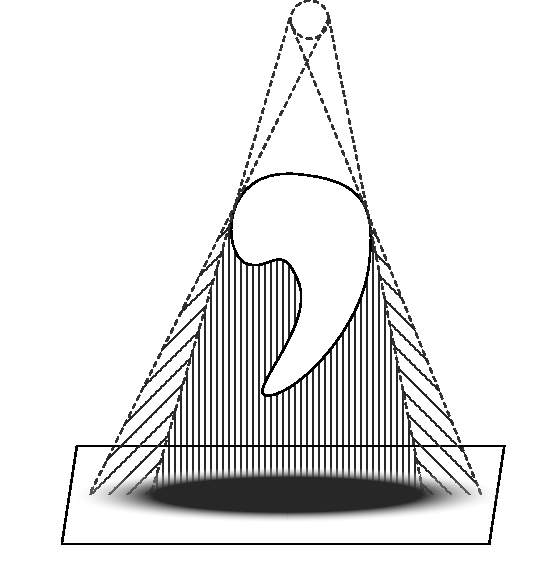
\includegraphics[width=0.5\textwidth]{./graf/shadow_example_soft.pdf}
    \caption{The umbra (under vertical lines) and penumbra (under slant lines) create a soft shadow.}
    \label{fig:shadow_soft}
\end{figure}

\subsection{Coarse distinction of shadow rendering techniques}

In this thesis a coarse distinction of the shadow rendering techniques into three groups is proposed. It is made based on the main mechanism utilized in a technique that defines which areas of the scene are in light and which are in shadow. Additionally, techniques in each group share similar issues that researches have attempted and are still attempting to resolve with newer iterations of the original algorithms.

The first group consists of image-based techniques.

Geometry-based

Ray-based

\subsection{Technique 1}
This is the first technique.

\subsection{Technique 2}
This is the second technique.

\subsection{Technique 3}
This is the third technique.

\subsection{Technique 4}

%%%%%%%%%%%%%%%%%%%%%%%%%%%%%%%%%%%%%%%%%%%%%%%%%%%%%%%%%%%%%%%%%%%%%%%%%%%%%%%%

\begin{itemize}
\item What problem do I want (have to :-) to solve?
\item Why the problem is important?
\item How do others solve the problem?
\item What are pros and cons of my solution?
\end{itemize}

References to 
book \cite{bib:book},
scientific papers in journals \cite{bib:article},
conference papers \cite{bib:conference},
and web pages \cite{bib:internet}.

Equations should be numbered:
\begin{align}
y = \frac{\partial x}{\partial t}
\end{align}

\begin{itemize}
\item problem analysis, problem statement
\item state of the art, literature research (all sources in the thesis have to be referenced, eg journal article \cite{bib:article} book \cite{bib:book}, conference paper \cite{bib:conference}, internet source \cite{bib:internet})
\item description of known solutions, algorithms
\item location of the thesis in scientific domain
\item The title of this chapter is similar to the title of the thesis.
\end{itemize}

\begin{Definition}\label{def:definition}
body of the definitions
\end{Definition}

\begin{Theorem}[optional name]\label{t:theorem}
body of the theorem
\end{Theorem}

\begin{Example}[optional name]\label{ex:example}
body of the example
\end{Example}

%%%%%%%%%%%%%%%%%%%%%%%%


